\section{Numerical Approach to the Variational Problem and Strong Formulation} \label{sec:SI-VPandFDM}
\tstk{fix this section's name once you decide what makes the cut. Also make a proper introduction here, or at least a lead-in.}

In this section we turn to numerical schemes for handling the variational problem \eqref{eq:SI-VarProb} and the strong formulation \eqref{eq:SI-BulkEqn}-\eqref{eq:SI-VertexCondition}.
For each formulation, we will outline the numerical scheme we have chosen to pursue and, importantly, the methods in which we can handle the non-standard integrals and gradients with respect to $\compMes$ numerically.
Where appropriate we will use the "cross-in-the-plane" geometry from the example in section \tstk{ref!!}, now equipped with $\compMes$, to illustrate the results of these methods.

\subsection{Variational Problem} \label{ssec:SI-VP}
We begin by examining the variational problem \eqref{eq:SI-VarProb},
\begin{align*} 
	\omega_n^2 &:= \min_{u}\clbracs{ \integral{\ddom}{ \abs{\tgrad_{\compMes}u}^2 }{\compMes} \setVert \norm{u}_{\ltwo{\ddom}{\compMes}}=1, \ u\perp u_l \ \forall 1\leq l\leq n-1 }. \tag{\eqref{eq:SI-VarProb} restated}
\end{align*}
\tstk{this is a fail safe, belongs when we talk about the numerical methods themselves.}
The equations \eqref{eq:SI-BulkEqn}-\eqref{eq:SI-VertexCondition} and variational problem \eqref{eq:SI-VarProb} of course provide us with the same eigenvalues and eigenfunctions, as can be deduced from applying the Lagrange multiplier theorem to \eqref{eq:SI-VarProb}. \tstk{do this maybe? See notes from 23-11-21.}
Our interest is in determining the eigenvalues $\omega_n^2$, however we also need to determine the eigenfunctions $u_n$ since we need $u_n$ to be orthogonal to each of $u_l, 1\leq l\leq n-1$.
Given that we can obtain the eigenvalue $\omega_n^2$ from the eigenfunction $u_n$ by evaluating the integral in \eqref{eq:SI-VarProb}, we will focus our discussion on the approximation (and computation) of the eigenfunctions.
We also drop the explicit subscript $n$, and just consider the problem of determining the function $u\in\tgradSob{\ddom}{\compMes}$ which solves the optimisation problem
\begin{subequations} \label{eq:SI-MinProblem}
	\begin{align}
		\text{Minimise} \quad & \quad \integral{\ddom}{ \abs{\tgrad_{\compMes}u}^2 }{\compMes} \\
		\text{Subject to} \quad & \quad \integral{\ddom}{ \abs{u}^2 }{\compMes} = 1, \\
		& \quad \integral{\ddom}{ u\cdot\overline{u}_l }{\compMes} = 0, \ 1\leq l\leq n-1,
	\end{align}
\end{subequations}
where $n\in\naturals$, $u_l, 1\leq l\leq n-1$ are given (pairwise) orthogonal functions.
The traditional idea when attempting to approximate a minimising function is to represent the minimising function $u$ in a basis $\clbracs{\varphi_m}_{m\in\naturals_0}\subset\tgradSob{\ddom}{\compMes}$, truncate the basis expansion at some index $M$,
\begin{align} \label{eq:SI-VPTruncatedBasis}
	u &\approx \sum_{m=0}^M u_m \varphi_m,
\end{align}
and solve the minimisation problem (that arises from substituting \eqref{eq:SI-VPTruncatedBasis} into \eqref{eq:SI-MinProblem}) in the coefficients of the basis expansion that remain --- the choice of $M$ determines the accuracy in the approximate eigenfunction (and hence eigenvalue).
This minimisation problem will be discrete (solving for the $M+1$ independent variables $u_m$), and can be handled using optimisation methods.

None of the steps above are prohibited for the problem \eqref{eq:SI-MinProblem}, and so we can proceed with the aforementioned ideas.
We will illustrate this implementation for the "cross-in-the-plane" geometry first introduced in \tstk{example reference --- note, we might already mention this in the intro to this section, so could potentially avoid repetition}\footnote{For convenience, we have translated the period cell by $\bracs{\recip{2},\recip{2}}$ with regards to how this geometry was handled in \tstk{ref}. This just allows us to avoid carrying additional constant terms around in our computations, and we would obtain the same results as if we didn't apply any translation.}; we take $\ddom=\left[0,1\right)^2$, and let $\graph$ be the period graph with a single vertex $v_0=\bracs{0,0}^\top$, and two ``looping" edges $I_h = \sqbracs{0,1}\times\clbracs{0}$, $I_v=\clbracs{0}\times\sqbracs{0,1}$.
Our first task is to decide on the basis functions $\varphi_m$ that we want to use to approximate $u$.
From the standpoint of accuracy (and typically speed) of the numerical solution there are several properties that it is desirable for this basis to have; orthonormality between the $\varphi_m$, similar shape to that expected of $u$, and of course periodicity.
This is where problems concerning the unfamiliar nature of our space $\tgradSob{\ddom}{\compMes}$ begin to arise, as the choice of basis is considerably more complex --- as choosing the behaviour of $\varphi_m$ in the bulk regions then restricts what $\varphi_m$ can do on the skeleton, and vice-versa. 
The geometry of the skeleton can also compound this issue, particularly if there are a large number of bulk regions $\ddom_i$, if they have irregular shapes, or if their shapes are significantly different (in terms of size or shape) from each other.
As a general approach, one can choose a basis in similar fashion to how this is done for finite element schemes; mesh $\ddom$ into a union of simplexes (usually triangles) by placing nodes $\tau_i$, ensuring that none of the simplexes straddle any parts of the skeleton (that is, the interior of a simplex never has non-empty intersection with part of the skeleton).
Then, use ``tent" or ``hat" functions centred on each node $\tau_i$ for the truncated basis functions $\varphi_m$.
This allows sufficient flexibility in the behaviour of $u$ on the edges and in the bulk regions, at the expense of requiring a new mesh for every new graph geometry.

Fortunately, the geometry of our ``cross-in-the-plane" example is rather simple, since the two edges $I_h, I_v$ are aligned with the coordinate axes.
This makes computing integrals on the skeleton much simpler, and traces from the bulk region can be computed with relative ease, so we can avoid taking the approach of meshing $\ddom$ as described above.
Instead, we can opt to choose a basis in a way more akin to spectral methods --- by choosing ``global" basis functions rather than the ``local" tent-basis functions that meshing $\ddom$ would utilise.
Combined with the fact that we only have one bulk region that spans the entire period cell, the natural candidate for our basis functions would be the 2D Fourier basis $\e^{2\pi\rmi(\alpha x + \beta y)}$.
These functions are orthogonal in $\ltwo{\ddom}{\compMes}$, have period cell $\ddom$, and on each of the edges of $\graph$ reduce to a 1D-Fourier series.
However, these functions also possess a continuous (in the sense of matching traces) normal derivative across the skeleton, which functions in $\tgradSob{\ddom}{\compMes}$ are not required to have, and so we cannot use the Fourier basis.
Instead, we will look to use 2D polynomials to approximate our function $u$, by taking $M\in\naturals$ and setting
\begin{align} \label{eq:2DPolyBasisDef}
	\varphi_m(x,y) &= x^{i_m} y^{j_m}, \quad m = j_m + Mi_m, \ i,j\in\clbracs{0,...,M-1}.
\end{align}
These functions are not periodic by definition, so we are required to add the additional constraints
\begin{align*}
	u\bracs{0,y} = u\bracs{1,y}, \ \forall y\in\sqbracs{0,1}, 
	\qquad 
	u\bracs{x,0} = u\bracs{x,1}, \ \forall x\in\sqbracs{0,1},
\end{align*}
to our minimisation problem to account for this.
With this choice of basis, and writing $U = \bracs{u_0,...,u_{M^2-1}}^\top$, we are tasked with solving the following problem.
\begin{problem}[Discrete Variational Problem] \label{prob:DiscVarProb}
	Let $M,N\in\naturals$ and $\varphi_m$ be as in \eqref{eq:2DPolyBasisDef}.
	Given coefficients $U_l=\bracs{u^l_0,...,u^l_{M^2-1}}^\top$ for $1\leq l\neq N-1$, find values $U=\bracs{u_0,...,u_{M^2-1}}^\top$ that:
	\begin{subequations} \label{eq:SI-ExampleMinProb}
		\begin{align}
			\text{Minimise} \quad & \quad J\sqbracs{U} := \sum_{m=0}^{M^2-1}\sum_{n=0}^{M^2-1}u_m\overline{u}_n\ip{\tgrad_{\compMes}\varphi_m}{\tgrad_{\compMes}\varphi_n}_{\ltwo{\ddom}{\compMes}^2} 
			\label{eq:SI-EMPObjectiveFn} \\
			\text{Subject to} \quad & \quad \sum_{m=0}^{M^2-1}\sum_{n=0}^{M^2-1}u_m\overline{u}_n\ip{\varphi_m}{\varphi_n}_{\ltwo{\ddom}{\compMes}} = 1, 
			\label{eq:SI-EMPNormConstraint} \\
			& \quad \sum_{i_m=1}^{M-1}u_{j_m+Mi_m} = 0, \ \forall j_m\in\clbracs{0,...,M-1}, 
			\label{eq:SI-EMPxPeriodicity} \\
			& \quad \sum_{j_m=1}^{M-1}u_{j_m+Mi_m} = 0, \ \forall i_m\in\clbracs{0,...,M-1},
			\label{eq:SI-EMPyPeriodicity} \\
			& \quad \sum_{m=0}^{M^2-1}\sum_{n=0}^{M^2-1}u_m\overline{u}^l_n\ip{\varphi_m}{\varphi_n}_{\ltwo{\ddom}{\compMes}} = 0, \ \forall 1\leq l\leq N-1.
			\label{eq:SI-EMPOrthogonality}
		\end{align}
	\end{subequations}
\end{problem}
The minimiser $U$ of problem \ref{prob:DiscVarProb} then provides our approximation of $u$, and we have that $\omega^2 \approx J[U]$.
Equation \eqref{eq:SI-EMPNormConstraint} is the norm constraint on the eigenfunction $u$, \eqref{eq:SI-EMPxPeriodicity} (respectively \eqref{eq:SI-EMPyPeriodicity}) are the constraints that ensure periodicity of the eigenfunction in the $x$ (respectively $y$) directions, and \eqref{eq:SI-EMPOrthogonality} forces $u$ to be orthogonal to the previously computed eigenfunctions $u^l$.
Due to the finite dimension of our problem (through the truncation at order $M$ for the functions $\varphi_m$), we are only ever able to compute approximations to the lowest $M^2 - \bracs{2M + 1} + 1$ eigenvalues due to the number of constraints in the problem \ref{prob:DiscVarProb}.

\tstk{time to display some nice figures, maybe some comparisons between the two methods etc? Could also do a run of this with $\alpha_3\neq0$ just to see what on earth happens!}

\subsection{Finite Difference Scheme} \label{ssec:FDMSingInc}
As an alternative to working directly from the variational problem \ref{prob:DiscVarProb}, we can instead choose to work from our ``strong formulation" \eqref{eq:SI-BulkEqn}-\eqref{eq:SI-VertexCondition}.
Before we do so, it is convenient to notice that we can move the ``trace" terms in \eqref{eq:SI-InclusionEqn} to the left-hand-side to obtain the slightly nicer (in terms of the numerics that follow) looking system
\begin{subequations} \label{eq:SI-FDMEquationsToDisc}
	\begin{align}
		-\laplacian_\qm u 
		&= \omega^2 u 
		&\text{in } \ddom_i, \label{eq:SI-FDMBulk} \\
		- \bracs{\diff{}{y} + \rmi\qm_{jk}}^2u^{(jk)}  - \bracs{\bracs{\grad u\cdot n_{jk}}^+ - \bracs{\grad u\cdot n_{jk}}^-}
		&= \omega^2 u^{(jk)},
		&\text{in } I_{jk}, \label{eq:SI-FDMSkeleton} \\
		\sum_l \bracs{\pdiff{}{n}+\rmi\qm_{jk_l}} u^{(jk_l)}(v_j) 
		&= 0 
		&\text{at } v_j\in\vertSet. \label{eq:SI-FDMVertex}
	\end{align}
\end{subequations}
We have now placed everything except terms involving the spectral parameter on the left hand side of \eqref{eq:SI-FDMEquationsToDisc}, and our goal now is to devise a numerical scheme to approximate the action of the ``operators" on the left-hand-side, and from that approximate the spectrum of the problem.

Our idea is as follows; we recognise that $u$ is twice differentiable (in the familiar, classical sense) in each of the bulk regions and along each of the skeleton edges, so we can look to to approximate the spectrum of our problem by approximating $u$ through a (somewhat n{\"i}ave) finite-difference approximation in each of the bulk regions and skeleton edges, and tying these ``region-wise" approximations together.
To this end, we take each of the bulk regions $\ddom_i$, and place nodes $\tau_j\in\overline{\ddom}_{i}$ appropriately, so as to write finite difference approximations for $\laplacian_{\qm}u$ at each node $\tau_j\in\ddom_i$.
Note that, since $u$ is not required to be differentiable (in the classical sense) across the skeleton, it is important that any finite difference approximation at $\tau_j$ only uses the values of $u$ at other nodes in $\overline{\ddom}_{i}$.
In placing nodes in $\overline{\ddom}_{i}$, we will also end up with nodes placed on the portion of the skeleton (and vertices) that form part of $\partial\ddom_i$.
Since $u$ is twice differentiable along the skeleton, the placement of these nodes allows us to derive finite-difference approximations for the derivatives in \eqref{eq:SI-FDMSkeleton}.
The traces of the normal derivates (in \eqref{eq:SI-FDMSkeleton}) can also be approximated via one-sided differences using suitable nodes from each of the adjacent bulk regions.
Finally, an approximation for \eqref{eq:SI-FDMVertex} can be derived for nodes that lie at vertices $v_j\in\vertSet$, using the nodes that lie on edges that connect to $v_j$.
We will come to discuss some of the difficulties with the general application of this procedure after our illustrative example.
For now, assuming we have approximations for the gradient- and derivative-like objects, we can then approximate the action of the left-hand-side of \eqref{eq:SI-FDMEquationsToDisc} via the action of a matrix $\mathcal{F}$ on the vector $U = \bracs{u_j}^\top$, where $u_j:=u\bracs{\tau_j}$.
As a result, we can then approximate the system \eqref{eq:SI-FDMEquationsToDisc} by the matrix-eigenvalue problem involving $\mathcal{F}$.

Let us begin by illustrating this approach using the ``cross in the plane" geometry \tstk{section ref}.
We first discretise $\ddom$ into a uniform mesh consisting of $N\times N$ nodes $\tau_{p,q} = \bracs{(p-1)h,(q-1)h}$ for $p,q\in\clbracs{1,...,N}$, with a mesh width of $h = \recip{N-1}$, and write $u_{p,q} = u\bracs{\tau_{p,q}}$.
It is important to note at this early stage that we can utilise a uniform mesh thanks to the rather simple geometry of the skeleton, and in general the meshing process will be more complex (see the discussion at the end of this section).
Note that there is no need to place nodes along both of the periodic edges of $\ddom$, so long as we keep track of which nodes are connected by periodicity, but for notational purposes it is convenient to include such nodes in our description.
Proceeding with the discretisation of the above equations, $u$ is twice differentiable in the bulk region $\ddom^{\circ}$, and so at points $\tau_{p,q}\not\in\graph$ we can discretise as
\begin{align*}
	-\laplacian_\qm u\bracs{\tau_{p,q}} &\approx 
	\bracs{\abs{\qm}^2 + 4h^{-2}}u_{p,q}
	-h^{-1}\bracs{h^{-1} + \rmi\qm_1}u_{p+1,q}
	-h^{-1}\bracs{h^{-1} - \rmi\qm_1}u_{p-1,q} \\
	&\qquad -h^{-1}\bracs{h^{-1} + \rmi\qm_2}u_{p,q+1}
	-h^{-1}\bracs{h^{-1} - \rmi\qm_2}u_{p,q-1}, \labelthis\label{eq:SI-FDMBulkDiscretise}
\end{align*}
using centred differences.
One can also use forward (also known as left) or backward (a.k.a right) differences to approximate the $\laplacian_{\qm}$ operator --- this will likely be necessary for more complex skeleton geometries as was hinted at previously.
Also worth noting is that, should one choose not to use (or be unable to use) a uniform mesh, one will still obtain a similar expression to \eqref{eq:SI-FDMBulkDiscretise} for the approximation of $\laplacian_\qm u$ at a node $\tau\not\in\graph$, but in terms of the values of $u$ at, and the distances to, the ``nearest neighbour" nodes to $\tau$.

For nodes $\tau_{p,q}\in I_{jk}$ (for either $I_{jk}=I_h$ or $I_v$), our finite difference approximations become slightly more complex as we are forced to consider the nearest nodes to $\tau_{p,q}$ that lie in the directions $e_{jk}$ and $n_{jk}$.
This is because $u$ is twice differentiable \emph{along the skeleton}, so we must approximate $\bracs{\diff{}{y} + \rmi\qm_{jk}}^2u^{(jk)}$ through finite differences along the edge $I_{jk}$, which will involve the values of $u$ at the nodes ``adjacent" to $\tau_{p,q}$ in the $e_{jk}$ and $-e_{jk}$ directions.
For the normal-derivative trace terms, we use one-sided finite differences to approximate these values at $\tau_{p,q}$, which involves the values of $u$ at the nodes ``adjacent" to $\tau_{p,q}$ in the $n_{jk}$ and $-n_{jk}$ directions.
For general skeleton geometries these requirements will contribute to the complications with meshing the domain, but since the edges are aligned with the coordinate axes in the cross-in-the-plane geometry, the vectors $e_{jk}$ and $n_{jk}$ are also aligned with the coordinate axes and the discretisation proceeds easily.
Those $\tau_{p,q}$ that lie on the horizontal edge $I_h$ have $q=\frac{N-1}{2}$ and $p\neq\frac{N-1}{2}$, so our finite difference approximation is
\begin{align*}
	- \bracs{\diff{}{y} + \rmi\qm_{jk}}^2u_{p,q} - \bracs{\bracs{\grad u_{p,q}\cdot n_{jk}}^+ - \bracs{\grad u_{p,q}\cdot n_{jk}}^-}
	& \approx \bracs{\qm_1^2 + 2h^{-1} + 2h^{-2}}u_{p,q} \\
	& \quad - h^{-1}\bracs{h^{-1} + \rmi\qm_1}u_{p+1,q} \\
	& \quad - h^{-1}\bracs{h^{-1} - \rmi\qm_1}u_{p-1,q} \\
	& \quad - h^{-1}u_{p,q+1} - h^{-1}u_{p,q-1}, \labelthis\label{eq:SI-FDMHorzEdgeDiscretise}
\end{align*}
(where we reiterate $q=\frac{N-1}{2}$ and $p\neq\frac{N-1}{2}$).
Here we have used centred differences along the edge $I_h$, identifying that the nodes $\tau_{p-1,q}, \tau_{p+1,q}$ are the adjacent nodes in the $x_1 (= e_h)$ direction.
The traces cause the introduction of the terms $u_{p,q-1}$ and $u_{p,q+1}$, since $-x_2 = n_h$.
Analogously, nodes $\tau_{p,q}$ on the vertical edge $I_v$ have $p=\frac{N-1}{2}$ and $q\neq\frac{N-1}{2}$, and the finite difference approximation is
\begin{align*}
	- \bracs{\diff{}{y} + \rmi\qm_{jk}}^2_{p,q} - \bracs{\bracs{\grad u_{p,q}\cdot n_{jk}}^+ - \bracs{\grad u_{p,q}\cdot n_{jk}}^-}
	& \approx \bracs{\qm_2^2 + 2h^{-1} + 2h^{-2}}u_{p,q} \\
	& \quad - h^{-1}\bracs{h^{-1} + \rmi\qm_2}u_{p,q+1} \\
	& \quad - h^{-1}\bracs{h^{-1} - \rmi\qm_2}u_{p,q-1} \\
	& \quad - h^{-1}u_{p+1,q} - h^{-1}u_{p-1,q}. \labelthis\label{eq:SI-FDMVertEdgeDiscretise}
\end{align*}

Finally, we come to the node $\tau_{\frac{N-1}{2},\frac{N-1}{2}}$ placed at the vertex $v_0$.
Our finite difference approximation already enforces that $u$ be continuous at $v_0$, so we just have to enforce the vertex condition at this node.
Here we again approximate each (signed) normal derivative by a one-sided finite difference from the adjacent edges, giving us
\begin{align} \label{eq:SI-FDMVertCond}
	\sum_{j\con k}\bracs{ \pdiff{}{n} + \rmi\qm_{jk} }u_{\frac{N-1}{2},\frac{N-1}{2}}
	&\approx h^{-1} \bracs{ 4u_{p,q} - u_{p+1,q} - u_{p-1,q} - u_{p,q+1} - u_{p,q-1} },
\end{align}
where $p = q = \frac{N-1}{2}$.
We now insert these finite difference approximations \eqref{eq:SI-FDMBulkDiscretise}-\eqref{eq:SI-FDMVertCond} into \eqref{eq:SI-FDMEquationsToDisc}, which provides the following system in the $\bracs{N-1}^2$ nodal values $u_{p,q}$;
\begin{subequations} \label{eq:SI-FDMDiscreteEqns}
	\begin{align*}
		\bracs{\abs{\qm}^2 + 4h^{-2}}u_{p,q} \\
		-h^{-1}\bracs{h^{-1} + \rmi\qm_1}u_{p+1,q}
		-h^{-1}\bracs{h^{-1} - \rmi\qm_1}u_{p-1,q} & & \\
		\quad -h^{-1}\bracs{h^{-1} + \rmi\qm_2}u_{p,q+1}
		-h^{-1}\bracs{h^{-1} - \rmi\qm_2}u_{p,q-1}
		& = \omega^2 u_{p,q}, &\quad p,q\neq\frac{N-1}{2}, \labelthis\label{eq:SI-FDMBulkDiscEqns} \\
		\bracs{\qm_1^2 + 2h^{-1} + 2h^{-2}}u_{p,q} \\
		- h^{-1}\bracs{h^{-1} + \rmi\qm_1}u_{p+1,q}
		- h^{-1}\bracs{h^{-1} - \rmi\qm_1}u_{p-1,q} & & \\
		\quad - h^{-1}u_{p,q+1} - h^{-1}u_{p,q-1}
		&= \omega^2 u_{p,q}, &\quad p\neq\frac{N-1}{2}, q=\frac{N-1}{2}, \labelthis\label{eq:SI-FDMHEdge} \\
		\bracs{\qm_2^2 + 2h^{-1} + 2h^{-2}}u_{p,q} \\
		- h^{-1}\bracs{h^{-1} + \rmi\qm_2}u_{p,q+1}
		- h^{-1}\bracs{h^{-1} - \rmi\qm_2}u_{p,q-1} & & \\
		- h^{-1}u_{p+1,q} - h^{-1}u_{p-1,q}
		&= \omega^2 u_{p,q}, &\quad p=\frac{N-1}{2}, q\neq\frac{N-1}{2}, \labelthis\label{eq:SI-FDMVEdge} \\
		h^{-1} \bracs{ 4u_{p,q} - u_{p+1,q} - u_{p-1,q} - u_{p,q+1} - u_{p,q-1} }
		&= 0, & p=q=\frac{N-1}{2}, \labelthis\label{eq:SI-FDMDiscVertex}
	\end{align*}
\end{subequations}
where $p,q\in\clbracs{0,...,N-1}$.
This system can then be written in matrix form as 
\begin{align} \label{eq:SI-FDMMatrixEqn}
	\mathcal{F}U &= \omega^2 B U,
\end{align}
where $B=\mathrm{diag}\bracs{1,...,1,0,1,...,1}$ is a (positive semi-definite) diagonal matrix with the zero in the row corresponding to the equation \eqref{eq:SI-FDMDiscVertex}.
The equation \eqref{eq:SI-FDMMatrixEqn} can then be solved using a generalised eigenvalue solver to obtain the approximate eigenvalues $\omega^2$ and eigenvectors $U$.

\tstk{this gives us the numerical results in the file \texttt{CompositeMedium\_PeriodicFDM.ipynb} - I can export the results we want to pdfs and import them as images here.
Things to note are that the finite-difference matrix $\mathcal{F}$ is not Hermitian, but the eigenvalues appear to all be real.
The eigenfunction plots are also quite nice, but we don't have anything to compare them to (true values, etc).
Comparison with the ``spectral" method is also a must, certainly for the results we have obtained --- maybe give the difference in spectral values found for a fixed theta, and varying the mesh width and $M$ (in VP)?
Also need to mention how we have wasted a lot of our effort in solving in the bulk regions, when in reality we don't actually need the form of the function here...}
The approximate eigenvalues computed by the finite difference scheme are displayed in figure \ref{fig:CompositeCross-FDM-SpectralBands}, using $N=251$ grid-points in each of the coordinate directions.
\begin{figure}[b!]
	\centering
	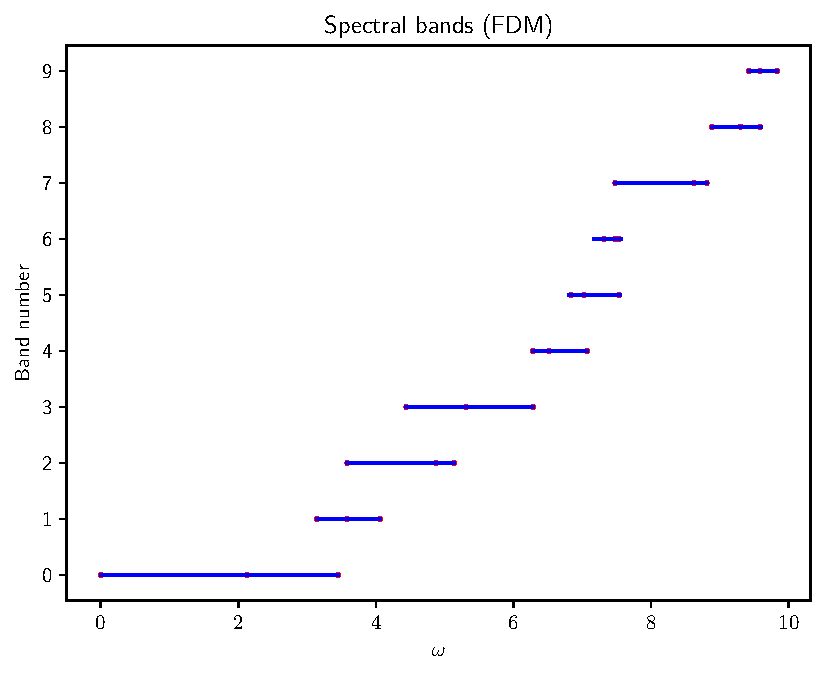
\includegraphics[scale=1.0]{CompositeCross-FDM-SpectralBands.pdf}
	\caption{\label{fig:CompositeCross-FDM-SpectralBands} The approximate eigenvalues computed by the finite-difference scheme, sorted into spectral bands for the cross-in-the-plane geometry. Eigenvalues corresponding to the extremities of the quasi-momentum are plotted in red.}
\end{figure}
Those points plotted in red correspond to eigenvalues that were computed at quasi-momentum values of $\bracs{0,0}^\top$, $\bracs{-\pi,0}^\top$, $\bracs{0,-\pi}^\top$, $\bracs{-\pi,-\pi}^\top$, from which we can observe that these points typically form the endpoints of each of the spectral bands.
A notable exception to this is band 6, for which the eigenvalues at the extremities of the band are not obtained at any of these quasi-momentum values.
However by examining the eigenvalues in this band as functions of $\qm$, \tstk{insert figure for band 6?}, it can be noticed that these extreme eigenvalues occur at quasi-momentum values where one of the components is either 0 (for the minimum values) or $-\pi$ (for the maximum values).
Furthermore, the eigenvalues in each band are symmetric in $\qm$, which we expected due to the symmetry of the cross-in-the-plane geometry.
\tstk{analytic solutions and convergence rates - maybe move the ``analytic solutions we know" to the first time we (re)-introduce the X-in-plane geometry?}
We can also illustrate the rate of convergence of this numerical scheme to some of the eigenvalues and eigenfunctions that we can compute analytically.
Observe that, for $n,m\in\naturals$ the function
\begin{align*}
	u_{n,m}(x) &= \e^{-\rmi\qm\cdot x}\sin\bracs{n\pi x_1}\sin\bracs{m\pi x_2},
\end{align*}
is an eigenfunction of the Dirichlet laplacian on $[0,1)^2$, and so solves \eqref{eq:SI-BulkEqn} with $\omega^2 = \bracs{n^2+m^2}\pi^2$ with $u=0$ on the skeleton.
In the event that both
\begin{itemize}
	\item ($n$ is even and $\qm_1=0$) or ($n$ is odd and $\qm_1=-\pi$),
	\item ($m$ is even and $\qm_2=0$) or ($m$ is odd and $\qm_2=-\pi$),
\end{itemize}
hold, then $u_{n,m}$ is also an eigenfunction of \eqref{eq:SI-BulkEqn}-\eqref{eq:SI-VertexCondition} with the same eigenvalue (this causes the trace terms in \eqref{eq:SI-InclusionEqn} to cancel each other). \tstk{this is relevant later when we try to reduce to the graph... as we've found a Dirichlet eigenfunction that solves our problem!}
In these cases, we expect that the error in the approximate eigenvalue is of the order of $N^-2$, since our scheme makes use of centred differences in the bulk region, and on the skeleton the eigenfunction should be identically zero.
Indeed, this is what we observe numerically for each $n,m$, as shown in figure \ref{}
\begin{figure}[h]
	\centering
	\begin{subfigure}[t]{0.35\textwidth}
		\centering
		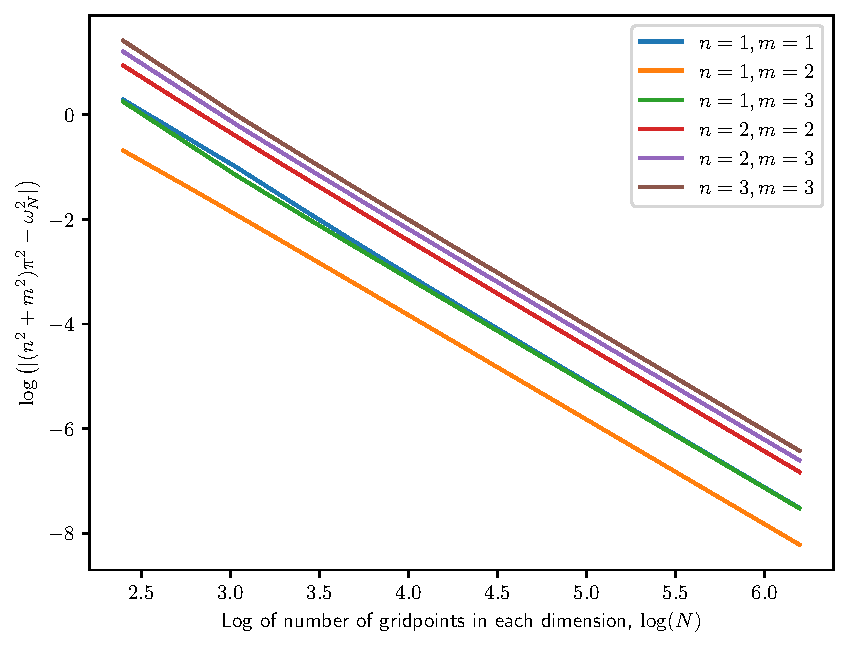
\includegraphics[scale=0.35]{CompositeCross-FDM-DEV-LogError.pdf}
		\caption{\label{fig:CompositeCross-FDM-DEV-LogError} Logarithm of the error in the eigenvalue $2\pi^2$ ($n=m=1$) computed by the finite difference approximation against $\log(N)$. The gradient of the slope is approximately $-2.004$.}
	\end{subfigure}
	~
	\begin{subfigure}[t]{0.65\textwidth}
		\centering
		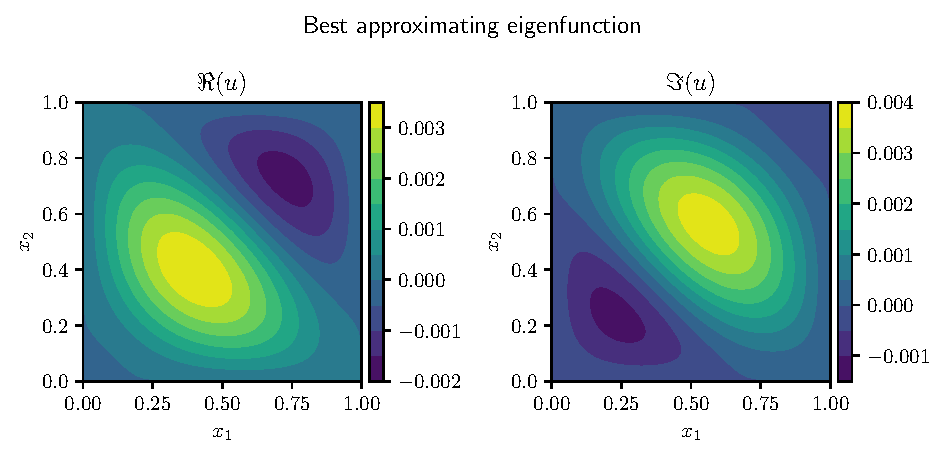
\includegraphics[scale=0.65]{CompositeCross-FDM-DEV-Function.pdf}
		\caption{\label{fig:CompositeCross-FDM-DEV-Function} The approximation to $u_{1,1}$ as computed by the finite difference scheme.}
	\end{subfigure}
	\caption{\label{fig:}}
\end{figure}
\tstk{plot titles need work. Also, spectral plot is causing much lag, maybe pdf output not the best?}

\tstk{now reflections on how this method might get much more complicated}
Our example using the cross-in-the-plane geometry illustrates the principle behind this approach; use finite differences to approximate $u$ in each $\ddom_i$ and along each $I_{jk}$, and tie approximations from adjacent bulk regions together through the nodal values along the common edge of the skeleton.
Compared to the variational approach in section \ref{ssec:SI-VP}, this approach avoids working with $\compMes$ directly and instead allows us to work solely in terms of classical derivatives, approximating them through Taylor's theorem.
However by choosing to approximate our function within each region and then ``stitch" these approximations together, we must choose our mesh in such a way as to abide by this decision, which can lead to some further considerations.
Let us begin by considering the requirements of the placement of nodes within the bulk regions --- each node must have neighbours in each of the coordinate directions that lie within the (closure of) the bulk region.
Now, consider a bulk region like that in figure \ref{fig:Diagram_FDMMeshIssue}, where a part of the skeleton is not aligned to the coordinate axes.
\begin{figure}[t]
	\centering
	\begin{subfigure}[t]{0.3\textwidth}
		\centering
		\includegraphics[scale=1.0]{Diagram_FDMMeshIssue-a.pdf}
		\caption{\label{fig:Diagram_FDMMeshIssue-a} A uniform mesh does not ensure that nodes in the bulk regions have neighbouring nodes which will provide us with a $C^2$-approximation, nor that every vertex has a node placed at it.}
	\end{subfigure}
	~
	\begin{subfigure}[t]{0.3\textwidth}
		\centering
		\includegraphics[scale=1.0]{Diagram_FDMMeshIssue-b.pdf}
		\caption{\label{fig:Diagram_FDMMeshIssue-b} Placing additional nodes along the skeleton edges, ensuring nodes in the bulk region have neighbours that lie within that same bulk region or on its boundary.}
	\end{subfigure}
	~
	\begin{subfigure}[t]{0.3\textwidth}
		\centering
		\includegraphics[scale=1.0]{Diagram_FDMMeshIssue-c.pdf}
		\caption{\label{fig:Diagram_FDMMeshIssue-c} The nearest nodes in the directions $\pm n_{jk}$ from the skeleton may be far from the edge or not exist at all (left highlighted node). Interpolation (right highlighted node) offers a solution, provided the bulk region is meshed well.}
	\end{subfigure}
	\caption{\label{fig:Diagram_FDMMeshIssue} An illustration of the complications encountered and considerations to be made when setting up a finite difference based approach for a general skeleton.}
\end{figure}
As we can quickly realise, uniform mesh will not be sufficient in this case, nor in general when the skeleton has edges that are not aligned to the coordinate axes. 
In figure \ref{fig:Diagram_FDMMeshIssue-a}, the highlighted node in the bulk region has no neighbour ``below" that lies within the same bulk region or its boundary, so a centred difference approximation to $\laplacian_{\qm}u$ at this node cannot be used.
One could argue that a suitable value for $u$ ``below" the highlighted node could be read off from interpolating values between nodes along the edge (then applying the knowledge that $u$ is continuous across the skeleton).
However there is no assurance that this interpolation will produce an accurate value for $u$, particularly if we are in the situation in figure \ref{fig:Diagram_FDMMeshIssue-a} where there are only two nodes along the diagonal edge, and the lower-left vertex doesn't even have a node placed at it.
To address this meshing complication, one can introduce additional nodes along the skeleton (and at the vertices) where necessary, as in figure \ref{fig:Diagram_FDMMeshIssue-b} (highlighted in blue).
This results in every node in the bulk regions having suitable neighbours in the coordinate directions, and has the additional bonus of improving the approximation of the derivative of $u$ along the skeleton.
Our expense is that we have given up a uniform distance between all nodes, which will require us to take slightly more care when deriving difference equations at each node and assembling the matrix $\mathcal{F}$.
We also may end up compounding another issue when we come to approximate the normal derivative traces in \eqref{eq:SI-FDMSkeleton}, which we highlight in figure \ref{fig:Diagram_FDMMeshIssue-c} --- if an edge is not aligned with the coordinate axes, where are the nearest nodes in the directions $\pm n_{jk}$ from the edge?
There is the possibility that such a node is far from the edge, again resulting in a poor approximation to the trace of the normal derivative, or that such a node may not even exist (see the leftmost highlighted node in figure \ref{fig:Diagram_FDMMeshIssue-c}).
We again have the option of interpolating a value for $u$ in the bulk regions, schematically illustrated at the right highlighted node in figure \ref{fig:Diagram_FDMMeshIssue-c} --- the values at the orange points can be interpolated from nodes in the bulk region, provided we have already made sensible mesh choices within the adjacent bulk regions\footnote{Note that we cannot simply decide to make the mesh in the bulk region finer, so that a node is placed in the position we want to interpolate. In general, doing so will end up in us requiring more nodes on the skeleton through the issue in figure \ref{fig:Diagram_FDMMeshIssue-a}, sending us in circles!}.
These issues arise due to how the skeleton (or more precisely, each edge of the skeleton) is effectively using a different coordinate system (for its derivatives) to the bulk regions, which is why this issue disappears when the edges of the skeleton are aligned to the coordinate axes --- the ``neighbouring" nodes we need on the skeleton are in the directions $e_{jk}, n_{jk}$ rather than the coordinate directions $x_1, x_2$.
Whilst the complications this brings can be combatted in the manners discussed above, it does highlight the need for care when setting up and implementing this approach for general skeleton geometries.
Contrastingly, the variational approach in \ref{ssec:SI-VP} does not run into these issues since (in that approach) we have made the choice to work with $\compMes$ directly and approximate the related gradients globally (over the whole domain) rather than utilising their properties on sub-regions.
\tstk{convergence experiments to the analytic solutions that we know about --- Dirichlet laplacian solutions...}

\tstk{could have a final paragraph or two commenting on a finite element based approach, which is a middle ground between the two approaches discussed here. It uses the variational form, but the basis functions that we'll be using would be local...}